\documentclass[twoside]{book}

% Packages required by doxygen
\usepackage{fixltx2e}
\usepackage{calc}
\usepackage{doxygen}
\usepackage[export]{adjustbox} % also loads graphicx
\usepackage{graphicx}
\usepackage[utf8]{inputenc}
\usepackage{makeidx}
\usepackage{multicol}
\usepackage{multirow}
\PassOptionsToPackage{warn}{textcomp}
\usepackage{textcomp}
\usepackage[nointegrals]{wasysym}
\usepackage[table]{xcolor}

% Font selection
\usepackage[T1]{fontenc}
\usepackage[scaled=.90]{helvet}
\usepackage{courier}
\usepackage{amssymb}
\usepackage{sectsty}
\renewcommand{\familydefault}{\sfdefault}
\allsectionsfont{%
  \fontseries{bc}\selectfont%
  \color{darkgray}%
}
\renewcommand{\DoxyLabelFont}{%
  \fontseries{bc}\selectfont%
  \color{darkgray}%
}
\newcommand{\+}{\discretionary{\mbox{\scriptsize$\hookleftarrow$}}{}{}}

% Page & text layout
\usepackage{geometry}
\geometry{%
  a4paper,%
  top=2.5cm,%
  bottom=2.5cm,%
  left=2.5cm,%
  right=2.5cm%
}
\tolerance=750
\hfuzz=15pt
\hbadness=750
\setlength{\emergencystretch}{15pt}
\setlength{\parindent}{0cm}
\setlength{\parskip}{0.2cm}
\makeatletter
\renewcommand{\paragraph}{%
  \@startsection{paragraph}{4}{0ex}{-1.0ex}{1.0ex}{%
    \normalfont\normalsize\bfseries\SS@parafont%
  }%
}
\renewcommand{\subparagraph}{%
  \@startsection{subparagraph}{5}{0ex}{-1.0ex}{1.0ex}{%
    \normalfont\normalsize\bfseries\SS@subparafont%
  }%
}
\makeatother

% Headers & footers
\usepackage{fancyhdr}
\pagestyle{fancyplain}
\fancyhead[LE]{\fancyplain{}{\bfseries\thepage}}
\fancyhead[CE]{\fancyplain{}{}}
\fancyhead[RE]{\fancyplain{}{\bfseries\leftmark}}
\fancyhead[LO]{\fancyplain{}{\bfseries\rightmark}}
\fancyhead[CO]{\fancyplain{}{}}
\fancyhead[RO]{\fancyplain{}{\bfseries\thepage}}
\fancyfoot[LE]{\fancyplain{}{}}
\fancyfoot[CE]{\fancyplain{}{}}
\fancyfoot[RE]{\fancyplain{}{\bfseries\scriptsize Generated on Sat Mar 12 2016 19\+:08\+:50 for Phone\+App by Doxygen }}
\fancyfoot[LO]{\fancyplain{}{\bfseries\scriptsize Generated on Sat Mar 12 2016 19\+:08\+:50 for Phone\+App by Doxygen }}
\fancyfoot[CO]{\fancyplain{}{}}
\fancyfoot[RO]{\fancyplain{}{}}
\renewcommand{\footrulewidth}{0.4pt}
\renewcommand{\chaptermark}[1]{%
  \markboth{#1}{}%
}
\renewcommand{\sectionmark}[1]{%
  \markright{\thesection\ #1}%
}

% Indices & bibliography
\usepackage{natbib}
\usepackage[titles]{tocloft}
\setcounter{tocdepth}{3}
\setcounter{secnumdepth}{5}
\makeindex

% Hyperlinks (required, but should be loaded last)
\usepackage{ifpdf}
\ifpdf
  \usepackage[pdftex,pagebackref=true]{hyperref}
\else
  \usepackage[ps2pdf,pagebackref=true]{hyperref}
\fi
\hypersetup{%
  colorlinks=true,%
  linkcolor=blue,%
  citecolor=blue,%
  unicode%
}

% Custom commands
\newcommand{\clearemptydoublepage}{%
  \newpage{\pagestyle{empty}\cleardoublepage}%
}


%===== C O N T E N T S =====

\begin{document}

% Titlepage & ToC
\hypersetup{pageanchor=false,
             bookmarks=true,
             bookmarksnumbered=true,
             pdfencoding=unicode
            }
\pagenumbering{roman}
\begin{titlepage}
\vspace*{7cm}
\begin{center}%
{\Large Phone\+App }\\
\vspace*{1cm}
{\large Generated by Doxygen 1.8.10}\\
\vspace*{0.5cm}
{\small Sat Mar 12 2016 19:08:50}\\
\end{center}
\end{titlepage}
\clearemptydoublepage
\tableofcontents
\clearemptydoublepage
\pagenumbering{arabic}
\hypersetup{pageanchor=true}

%--- Begin generated contents ---
\chapter{Namespace Index}
\section{Packages}
Here are the packages with brief descriptions (if available)\+:\begin{DoxyCompactList}
\item\contentsline{section}{\hyperlink{namespacecourse}{course} }{\pageref{namespacecourse}}{}
\item\contentsline{section}{\hyperlink{namespacecourse_1_1examples}{course.\+examples} }{\pageref{namespacecourse_1_1examples}}{}
\item\contentsline{section}{\hyperlink{namespacecourse_1_1examples_1_1phoneapp}{course.\+examples.\+phoneapp} }{\pageref{namespacecourse_1_1examples_1_1phoneapp}}{}
\end{DoxyCompactList}

\chapter{Hierarchical Index}
\section{Class Hierarchy}
This inheritance list is sorted roughly, but not completely, alphabetically\+:\begin{DoxyCompactList}
\item \contentsline{section}{course.\+examples.\+phoneapp.\+Constants}{\pageref{interfacecourse_1_1examples_1_1phoneapp_1_1_constants}}{}
\item \contentsline{section}{course.\+examples.\+phoneapp.\+Contact\+\_\+\+Details}{\pageref{classcourse_1_1examples_1_1phoneapp_1_1_contact___details}}{}
\item \contentsline{section}{course.\+examples.\+phoneapp.\+Shake\+Listener.\+On\+Shake\+Listener}{\pageref{interfacecourse_1_1examples_1_1phoneapp_1_1_shake_listener_1_1_on_shake_listener}}{}
\item \contentsline{section}{course.\+examples.\+phoneapp.\+Utility}{\pageref{classcourse_1_1examples_1_1phoneapp_1_1_utility}}{}
\item Activity\begin{DoxyCompactList}
\item \contentsline{section}{course.\+examples.\+phoneapp.\+Main\+Activity}{\pageref{classcourse_1_1examples_1_1phoneapp_1_1_main_activity}}{}
\item \contentsline{section}{course.\+examples.\+phoneapp.\+Ops\+Activity}{\pageref{classcourse_1_1examples_1_1phoneapp_1_1_ops_activity}}{}
\end{DoxyCompactList}
\item Sensor\+Event\+Listener\begin{DoxyCompactList}
\item \contentsline{section}{course.\+examples.\+phoneapp.\+Shake\+Listener}{\pageref{classcourse_1_1examples_1_1phoneapp_1_1_shake_listener}}{}
\end{DoxyCompactList}
\end{DoxyCompactList}

\chapter{Class Index}
\section{Class List}
Here are the classes, structs, unions and interfaces with brief descriptions\+:\begin{DoxyCompactList}
\item\contentsline{section}{\hyperlink{interfacecourse_1_1examples_1_1phoneapp_1_1_constants}{course.\+examples.\+phoneapp.\+Constants} }{\pageref{interfacecourse_1_1examples_1_1phoneapp_1_1_constants}}{}
\item\contentsline{section}{\hyperlink{classcourse_1_1examples_1_1phoneapp_1_1_contact___details}{course.\+examples.\+phoneapp.\+Contact\+\_\+\+Details} }{\pageref{classcourse_1_1examples_1_1phoneapp_1_1_contact___details}}{}
\item\contentsline{section}{\hyperlink{classcourse_1_1examples_1_1phoneapp_1_1_main_activity}{course.\+examples.\+phoneapp.\+Main\+Activity} }{\pageref{classcourse_1_1examples_1_1phoneapp_1_1_main_activity}}{}
\item\contentsline{section}{\hyperlink{interfacecourse_1_1examples_1_1phoneapp_1_1_shake_listener_1_1_on_shake_listener}{course.\+examples.\+phoneapp.\+Shake\+Listener.\+On\+Shake\+Listener} }{\pageref{interfacecourse_1_1examples_1_1phoneapp_1_1_shake_listener_1_1_on_shake_listener}}{}
\item\contentsline{section}{\hyperlink{classcourse_1_1examples_1_1phoneapp_1_1_ops_activity}{course.\+examples.\+phoneapp.\+Ops\+Activity} }{\pageref{classcourse_1_1examples_1_1phoneapp_1_1_ops_activity}}{}
\item\contentsline{section}{\hyperlink{classcourse_1_1examples_1_1phoneapp_1_1_shake_listener}{course.\+examples.\+phoneapp.\+Shake\+Listener} }{\pageref{classcourse_1_1examples_1_1phoneapp_1_1_shake_listener}}{}
\item\contentsline{section}{\hyperlink{classcourse_1_1examples_1_1phoneapp_1_1_utility}{course.\+examples.\+phoneapp.\+Utility} }{\pageref{classcourse_1_1examples_1_1phoneapp_1_1_utility}}{}
\end{DoxyCompactList}

\chapter{File Index}
\section{File List}
Here is a list of all files with brief descriptions\+:\begin{DoxyCompactList}
\item\contentsline{section}{app/src/main/java/course/examples/phoneapp/\hyperlink{_constants_8java}{Constants.\+java} }{\pageref{_constants_8java}}{}
\item\contentsline{section}{app/src/main/java/course/examples/phoneapp/\hyperlink{_contact___details_8java}{Contact\+\_\+\+Details.\+java} }{\pageref{_contact___details_8java}}{}
\item\contentsline{section}{app/src/main/java/course/examples/phoneapp/\hyperlink{_main_activity_8java}{Main\+Activity.\+java} }{\pageref{_main_activity_8java}}{}
\item\contentsline{section}{app/src/main/java/course/examples/phoneapp/\hyperlink{_ops_activity_8java}{Ops\+Activity.\+java} }{\pageref{_ops_activity_8java}}{}
\item\contentsline{section}{app/src/main/java/course/examples/phoneapp/\hyperlink{_shake_listener_8java}{Shake\+Listener.\+java} }{\pageref{_shake_listener_8java}}{}
\item\contentsline{section}{app/src/main/java/course/examples/phoneapp/\hyperlink{_utility_8java}{Utility.\+java} }{\pageref{_utility_8java}}{}
\end{DoxyCompactList}

\chapter{Namespace Documentation}
\hypertarget{namespacecourse}{}\section{Package course}
\label{namespacecourse}\index{course@{course}}
\subsection*{Packages}
\begin{DoxyCompactItemize}
\item 
package \hyperlink{namespacecourse_1_1examples}{examples}
\end{DoxyCompactItemize}

\hypertarget{namespacecourse_1_1examples}{}\section{Package course.\+examples}
\label{namespacecourse_1_1examples}\index{course.\+examples@{course.\+examples}}
\subsection*{Packages}
\begin{DoxyCompactItemize}
\item 
package \hyperlink{namespacecourse_1_1examples_1_1phoneapp}{phoneapp}
\end{DoxyCompactItemize}

\hypertarget{namespacecourse_1_1examples_1_1phoneapp}{}\section{Package course.\+examples.\+phoneapp}
\label{namespacecourse_1_1examples_1_1phoneapp}\index{course.\+examples.\+phoneapp@{course.\+examples.\+phoneapp}}
\subsection*{Classes}
\begin{DoxyCompactItemize}
\item 
interface \hyperlink{interfacecourse_1_1examples_1_1phoneapp_1_1_constants}{Constants}
\item 
class \hyperlink{classcourse_1_1examples_1_1phoneapp_1_1_contact___details}{Contact\+\_\+\+Details}
\item 
class \hyperlink{classcourse_1_1examples_1_1phoneapp_1_1_main_activity}{Main\+Activity}
\item 
class \hyperlink{classcourse_1_1examples_1_1phoneapp_1_1_ops_activity}{Ops\+Activity}
\item 
class \hyperlink{classcourse_1_1examples_1_1phoneapp_1_1_shake_listener}{Shake\+Listener}
\item 
class \hyperlink{classcourse_1_1examples_1_1phoneapp_1_1_utility}{Utility}
\end{DoxyCompactItemize}

\chapter{Class Documentation}
\hypertarget{classcourse_1_1examples_1_1phoneapp_1_1_contact___details}{}\section{course.\+examples.\+phoneapp.\+Contact\+\_\+\+Details Class Reference}
\label{classcourse_1_1examples_1_1phoneapp_1_1_contact___details}\index{course.\+examples.\+phoneapp.\+Contact\+\_\+\+Details@{course.\+examples.\+phoneapp.\+Contact\+\_\+\+Details}}


\subsection{Detailed Description}
Created by kannanb on 2/22/2016. 

The documentation for this class was generated from the following file\+:\begin{DoxyCompactItemize}
\item 
app/src/main/java/course/examples/phoneapp/\hyperlink{_contact___details_8java}{Contact\+\_\+\+Details.\+java}\end{DoxyCompactItemize}

\hypertarget{classcourse_1_1examples_1_1phoneapp_1_1_main_activity}{}\section{course.\+examples.\+phoneapp.\+Main\+Activity Class Reference}
\label{classcourse_1_1examples_1_1phoneapp_1_1_main_activity}\index{course.\+examples.\+phoneapp.\+Main\+Activity@{course.\+examples.\+phoneapp.\+Main\+Activity}}


Inheritance diagram for course.\+examples.\+phoneapp.\+Main\+Activity\+:
\nopagebreak
\begin{figure}[H]
\begin{center}
\leavevmode
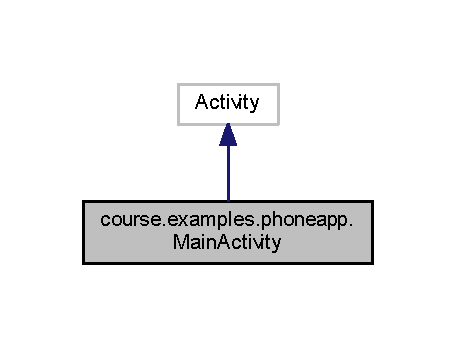
\includegraphics[width=219pt]{classcourse_1_1examples_1_1phoneapp_1_1_main_activity__inherit__graph}
\end{center}
\end{figure}


Collaboration diagram for course.\+examples.\+phoneapp.\+Main\+Activity\+:
\nopagebreak
\begin{figure}[H]
\begin{center}
\leavevmode
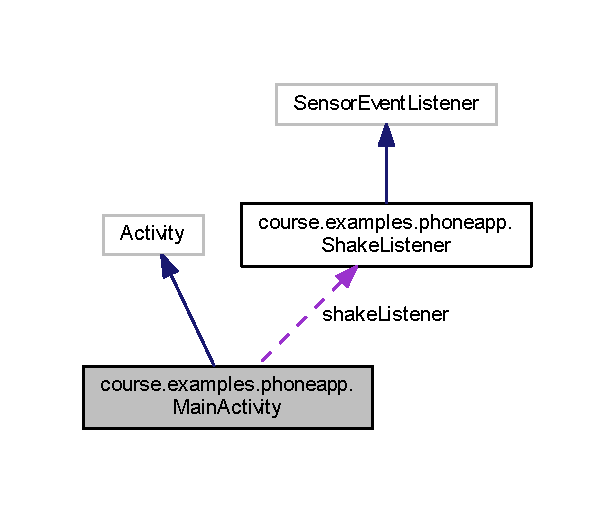
\includegraphics[width=284pt]{classcourse_1_1examples_1_1phoneapp_1_1_main_activity__coll__graph}
\end{center}
\end{figure}
\subsection*{Public Attributes}
\begin{DoxyCompactItemize}
\item 
String \hyperlink{classcourse_1_1examples_1_1phoneapp_1_1_main_activity_a2e49349c76e07dceda2b968b25b2f12e}{phone\+Details} = \char`\"{}\char`\"{}
\end{DoxyCompactItemize}
\subsection*{Static Public Attributes}
\begin{DoxyCompactItemize}
\item 
static final String \hyperlink{classcourse_1_1examples_1_1phoneapp_1_1_main_activity_a60a240e7bcd23f7fa0b2c9e78d19fffb}{P\+H\+O\+N\+E\+\_\+\+C\+O\+N\+T\+A\+C\+T\+S} = \char`\"{}contacts\char`\"{}
\item 
static final String \hyperlink{classcourse_1_1examples_1_1phoneapp_1_1_main_activity_a4c02f85155813ea9b9c5951f21474bea}{L\+O\+G\+\_\+\+T\+A\+G\+\_\+\+N\+A\+M\+E} = \char`\"{}Phone\+App.\+Main\+Activity\char`\"{}
\item 
static final Hash\+Map$<$ Integer, String $>$ \hyperlink{classcourse_1_1examples_1_1phoneapp_1_1_main_activity_a2b0ca4e6cb7439dbf892e504baa83c14}{phone\+Type\+Map} = new Hash\+Map$<$Integer, String$>$()
\end{DoxyCompactItemize}
\subsection*{Protected Member Functions}
\begin{DoxyCompactItemize}
\item 
void \hyperlink{classcourse_1_1examples_1_1phoneapp_1_1_main_activity_a070a6d5a698190ad3ccd4029ef0de81c}{on\+Create} (Bundle saved\+Instance\+State)
\end{DoxyCompactItemize}


\subsection{Detailed Description}
Main activity class for launching the U\+I containing all phone contacts on the device 

\subsection{Member Function Documentation}
\hypertarget{classcourse_1_1examples_1_1phoneapp_1_1_main_activity_a070a6d5a698190ad3ccd4029ef0de81c}{}\index{course\+::examples\+::phoneapp\+::\+Main\+Activity@{course\+::examples\+::phoneapp\+::\+Main\+Activity}!on\+Create@{on\+Create}}
\index{on\+Create@{on\+Create}!course\+::examples\+::phoneapp\+::\+Main\+Activity@{course\+::examples\+::phoneapp\+::\+Main\+Activity}}
\subsubsection[{on\+Create(\+Bundle saved\+Instance\+State)}]{\setlength{\rightskip}{0pt plus 5cm}void course.\+examples.\+phoneapp.\+Main\+Activity.\+on\+Create (
\begin{DoxyParamCaption}
\item[{Bundle}]{saved\+Instance\+State}
\end{DoxyParamCaption}
)\hspace{0.3cm}{\ttfamily [protected]}}\label{classcourse_1_1examples_1_1phoneapp_1_1_main_activity_a070a6d5a698190ad3ccd4029ef0de81c}
Initialize the U\+I component and the data structures defined in this class 
\begin{DoxyParams}{Parameters}
{\em saved\+Instance\+State} & \\
\hline
\end{DoxyParams}


\subsection{Member Data Documentation}
\hypertarget{classcourse_1_1examples_1_1phoneapp_1_1_main_activity_a4c02f85155813ea9b9c5951f21474bea}{}\index{course\+::examples\+::phoneapp\+::\+Main\+Activity@{course\+::examples\+::phoneapp\+::\+Main\+Activity}!L\+O\+G\+\_\+\+T\+A\+G\+\_\+\+N\+A\+M\+E@{L\+O\+G\+\_\+\+T\+A\+G\+\_\+\+N\+A\+M\+E}}
\index{L\+O\+G\+\_\+\+T\+A\+G\+\_\+\+N\+A\+M\+E@{L\+O\+G\+\_\+\+T\+A\+G\+\_\+\+N\+A\+M\+E}!course\+::examples\+::phoneapp\+::\+Main\+Activity@{course\+::examples\+::phoneapp\+::\+Main\+Activity}}
\subsubsection[{L\+O\+G\+\_\+\+T\+A\+G\+\_\+\+N\+A\+M\+E}]{\setlength{\rightskip}{0pt plus 5cm}final String course.\+examples.\+phoneapp.\+Main\+Activity.\+L\+O\+G\+\_\+\+T\+A\+G\+\_\+\+N\+A\+M\+E = \char`\"{}Phone\+App.\+Main\+Activity\char`\"{}\hspace{0.3cm}{\ttfamily [static]}}\label{classcourse_1_1examples_1_1phoneapp_1_1_main_activity_a4c02f85155813ea9b9c5951f21474bea}
\hypertarget{classcourse_1_1examples_1_1phoneapp_1_1_main_activity_a60a240e7bcd23f7fa0b2c9e78d19fffb}{}\index{course\+::examples\+::phoneapp\+::\+Main\+Activity@{course\+::examples\+::phoneapp\+::\+Main\+Activity}!P\+H\+O\+N\+E\+\_\+\+C\+O\+N\+T\+A\+C\+T\+S@{P\+H\+O\+N\+E\+\_\+\+C\+O\+N\+T\+A\+C\+T\+S}}
\index{P\+H\+O\+N\+E\+\_\+\+C\+O\+N\+T\+A\+C\+T\+S@{P\+H\+O\+N\+E\+\_\+\+C\+O\+N\+T\+A\+C\+T\+S}!course\+::examples\+::phoneapp\+::\+Main\+Activity@{course\+::examples\+::phoneapp\+::\+Main\+Activity}}
\subsubsection[{P\+H\+O\+N\+E\+\_\+\+C\+O\+N\+T\+A\+C\+T\+S}]{\setlength{\rightskip}{0pt plus 5cm}final String course.\+examples.\+phoneapp.\+Main\+Activity.\+P\+H\+O\+N\+E\+\_\+\+C\+O\+N\+T\+A\+C\+T\+S = \char`\"{}contacts\char`\"{}\hspace{0.3cm}{\ttfamily [static]}}\label{classcourse_1_1examples_1_1phoneapp_1_1_main_activity_a60a240e7bcd23f7fa0b2c9e78d19fffb}
\hypertarget{classcourse_1_1examples_1_1phoneapp_1_1_main_activity_a2e49349c76e07dceda2b968b25b2f12e}{}\index{course\+::examples\+::phoneapp\+::\+Main\+Activity@{course\+::examples\+::phoneapp\+::\+Main\+Activity}!phone\+Details@{phone\+Details}}
\index{phone\+Details@{phone\+Details}!course\+::examples\+::phoneapp\+::\+Main\+Activity@{course\+::examples\+::phoneapp\+::\+Main\+Activity}}
\subsubsection[{phone\+Details}]{\setlength{\rightskip}{0pt plus 5cm}String course.\+examples.\+phoneapp.\+Main\+Activity.\+phone\+Details = \char`\"{}\char`\"{}}\label{classcourse_1_1examples_1_1phoneapp_1_1_main_activity_a2e49349c76e07dceda2b968b25b2f12e}
\hypertarget{classcourse_1_1examples_1_1phoneapp_1_1_main_activity_a2b0ca4e6cb7439dbf892e504baa83c14}{}\index{course\+::examples\+::phoneapp\+::\+Main\+Activity@{course\+::examples\+::phoneapp\+::\+Main\+Activity}!phone\+Type\+Map@{phone\+Type\+Map}}
\index{phone\+Type\+Map@{phone\+Type\+Map}!course\+::examples\+::phoneapp\+::\+Main\+Activity@{course\+::examples\+::phoneapp\+::\+Main\+Activity}}
\subsubsection[{phone\+Type\+Map}]{\setlength{\rightskip}{0pt plus 5cm}final Hash\+Map$<$Integer, String$>$ course.\+examples.\+phoneapp.\+Main\+Activity.\+phone\+Type\+Map = new Hash\+Map$<$Integer, String$>$()\hspace{0.3cm}{\ttfamily [static]}}\label{classcourse_1_1examples_1_1phoneapp_1_1_main_activity_a2b0ca4e6cb7439dbf892e504baa83c14}


The documentation for this class was generated from the following file\+:\begin{DoxyCompactItemize}
\item 
app/src/main/java/course/examples/phoneapp/\hyperlink{_main_activity_8java}{Main\+Activity.\+java}\end{DoxyCompactItemize}

\hypertarget{interfacecourse_1_1examples_1_1phoneapp_1_1_shake_listener_1_1_on_shake_listener}{}\section{course.\+examples.\+phoneapp.\+Shake\+Listener.\+On\+Shake\+Listener Interface Reference}
\label{interfacecourse_1_1examples_1_1phoneapp_1_1_shake_listener_1_1_on_shake_listener}\index{course.\+examples.\+phoneapp.\+Shake\+Listener.\+On\+Shake\+Listener@{course.\+examples.\+phoneapp.\+Shake\+Listener.\+On\+Shake\+Listener}}
\subsection*{Public Member Functions}
\begin{DoxyCompactItemize}
\item 
void \hyperlink{interfacecourse_1_1examples_1_1phoneapp_1_1_shake_listener_1_1_on_shake_listener_ad1e4228d1fc44312e48e59f272ba6c4e}{on\+Shake} ()
\end{DoxyCompactItemize}


\subsection{Member Function Documentation}
\hypertarget{interfacecourse_1_1examples_1_1phoneapp_1_1_shake_listener_1_1_on_shake_listener_ad1e4228d1fc44312e48e59f272ba6c4e}{}\index{course\+::examples\+::phoneapp\+::\+Shake\+Listener\+::\+On\+Shake\+Listener@{course\+::examples\+::phoneapp\+::\+Shake\+Listener\+::\+On\+Shake\+Listener}!on\+Shake@{on\+Shake}}
\index{on\+Shake@{on\+Shake}!course\+::examples\+::phoneapp\+::\+Shake\+Listener\+::\+On\+Shake\+Listener@{course\+::examples\+::phoneapp\+::\+Shake\+Listener\+::\+On\+Shake\+Listener}}
\subsubsection[{on\+Shake()}]{\setlength{\rightskip}{0pt plus 5cm}void course.\+examples.\+phoneapp.\+Shake\+Listener.\+On\+Shake\+Listener.\+on\+Shake (
\begin{DoxyParamCaption}
{}
\end{DoxyParamCaption}
)}\label{interfacecourse_1_1examples_1_1phoneapp_1_1_shake_listener_1_1_on_shake_listener_ad1e4228d1fc44312e48e59f272ba6c4e}


The documentation for this interface was generated from the following file\+:\begin{DoxyCompactItemize}
\item 
app/src/main/java/course/examples/phoneapp/\hyperlink{_shake_listener_8java}{Shake\+Listener.\+java}\end{DoxyCompactItemize}

\hypertarget{classcourse_1_1examples_1_1phoneapp_1_1_ops_activity}{}\section{course.\+examples.\+phoneapp.\+Ops\+Activity Class Reference}
\label{classcourse_1_1examples_1_1phoneapp_1_1_ops_activity}\index{course.\+examples.\+phoneapp.\+Ops\+Activity@{course.\+examples.\+phoneapp.\+Ops\+Activity}}


Inheritance diagram for course.\+examples.\+phoneapp.\+Ops\+Activity\+:
\nopagebreak
\begin{figure}[H]
\begin{center}
\leavevmode
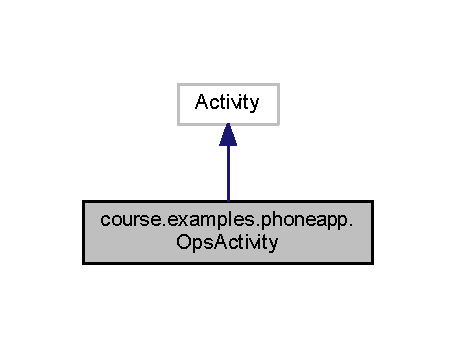
\includegraphics[width=219pt]{classcourse_1_1examples_1_1phoneapp_1_1_ops_activity__inherit__graph}
\end{center}
\end{figure}


Collaboration diagram for course.\+examples.\+phoneapp.\+Ops\+Activity\+:
\nopagebreak
\begin{figure}[H]
\begin{center}
\leavevmode
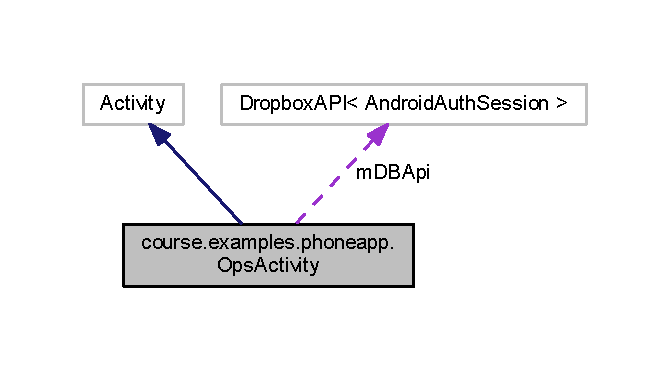
\includegraphics[width=322pt]{classcourse_1_1examples_1_1phoneapp_1_1_ops_activity__coll__graph}
\end{center}
\end{figure}
\subsection*{Public Member Functions}
\begin{DoxyCompactItemize}
\item 
void \hyperlink{classcourse_1_1examples_1_1phoneapp_1_1_ops_activity_a4483070d81483a14c450c03a23521b33}{retrieve\+Phone\+List} ()
\item 
void \hyperlink{classcourse_1_1examples_1_1phoneapp_1_1_ops_activity_a427848e2c42eb538b888f8b7214b8cd4}{perform\+Operation} ()
\item 
void \hyperlink{classcourse_1_1examples_1_1phoneapp_1_1_ops_activity_a55825f56d10a878fc5516121f0eda3bf}{set\+Tool\+Tips} ()
\item 
void \hyperlink{classcourse_1_1examples_1_1phoneapp_1_1_ops_activity_ae6f21dd987eba779e66e4bb66bbee391}{do\+Dropbox\+Authentication} ()
\item 
void \hyperlink{classcourse_1_1examples_1_1phoneapp_1_1_ops_activity_a329fad70246e569c6746b7a38f35e6e6}{on\+Create\+Context\+Menu} (Context\+Menu menu, View v, Context\+Menu.\+Context\+Menu\+Info menu\+Info)
\item 
boolean \hyperlink{classcourse_1_1examples_1_1phoneapp_1_1_ops_activity_a1c9753b2bbe4cf6d37c17f3a97df304b}{on\+Create\+Options\+Menu} (Menu menu)
\item 
boolean \hyperlink{classcourse_1_1examples_1_1phoneapp_1_1_ops_activity_a6175dfaf6290e9c3a13da40e5ef61e60}{on\+Options\+Item\+Selected} (Menu\+Item item)
\end{DoxyCompactItemize}
\subsection*{Public Attributes}
\begin{DoxyCompactItemize}
\item 
Dropbox\+A\+P\+I$<$ Android\+Auth\+Session $>$ \hyperlink{classcourse_1_1examples_1_1phoneapp_1_1_ops_activity_afa9dcbfe8d531688656b8ee3042ccba6}{m\+D\+B\+Api} = null
\end{DoxyCompactItemize}
\subsection*{Static Public Attributes}
\begin{DoxyCompactItemize}
\item 
static final String \hyperlink{classcourse_1_1examples_1_1phoneapp_1_1_ops_activity_a6bbe27893d347a4f66c9bac0e2dcc80b}{P\+H\+O\+N\+E\+\_\+\+C\+O\+N\+T\+A\+C\+T\+S} = \char`\"{}contacts\char`\"{}
\item 
static final String \hyperlink{classcourse_1_1examples_1_1phoneapp_1_1_ops_activity_ac2c7991a146c46106d21d22d1896ec35}{D\+R\+O\+P\+B\+O\+X\+\_\+\+N\+A\+M\+E} = \char`\"{}Drop\+Box-\/Contact\char`\"{}
\end{DoxyCompactItemize}
\subsection*{Protected Member Functions}
\begin{DoxyCompactItemize}
\item 
void \hyperlink{classcourse_1_1examples_1_1phoneapp_1_1_ops_activity_a124a97ed5678d96f0888b55db9e283bb}{on\+Create} (Bundle saved\+Instance\+State)
\item 
void \hyperlink{classcourse_1_1examples_1_1phoneapp_1_1_ops_activity_aeb8480322291f8d86c1afd370f4d46e9}{on\+Resume} ()
\item 
void \hyperlink{classcourse_1_1examples_1_1phoneapp_1_1_ops_activity_ae68d43a22b46dd1dea9f23b8f48589aa}{on\+Pause} ()
\end{DoxyCompactItemize}


\subsection{Detailed Description}
Created by kannanb on 2/21/2016. 

\subsection{Member Function Documentation}
\hypertarget{classcourse_1_1examples_1_1phoneapp_1_1_ops_activity_ae6f21dd987eba779e66e4bb66bbee391}{}\index{course\+::examples\+::phoneapp\+::\+Ops\+Activity@{course\+::examples\+::phoneapp\+::\+Ops\+Activity}!do\+Dropbox\+Authentication@{do\+Dropbox\+Authentication}}
\index{do\+Dropbox\+Authentication@{do\+Dropbox\+Authentication}!course\+::examples\+::phoneapp\+::\+Ops\+Activity@{course\+::examples\+::phoneapp\+::\+Ops\+Activity}}
\subsubsection[{do\+Dropbox\+Authentication()}]{\setlength{\rightskip}{0pt plus 5cm}void course.\+examples.\+phoneapp.\+Ops\+Activity.\+do\+Dropbox\+Authentication (
\begin{DoxyParamCaption}
{}
\end{DoxyParamCaption}
)}\label{classcourse_1_1examples_1_1phoneapp_1_1_ops_activity_ae6f21dd987eba779e66e4bb66bbee391}
\hypertarget{classcourse_1_1examples_1_1phoneapp_1_1_ops_activity_a124a97ed5678d96f0888b55db9e283bb}{}\index{course\+::examples\+::phoneapp\+::\+Ops\+Activity@{course\+::examples\+::phoneapp\+::\+Ops\+Activity}!on\+Create@{on\+Create}}
\index{on\+Create@{on\+Create}!course\+::examples\+::phoneapp\+::\+Ops\+Activity@{course\+::examples\+::phoneapp\+::\+Ops\+Activity}}
\subsubsection[{on\+Create(\+Bundle saved\+Instance\+State)}]{\setlength{\rightskip}{0pt plus 5cm}void course.\+examples.\+phoneapp.\+Ops\+Activity.\+on\+Create (
\begin{DoxyParamCaption}
\item[{Bundle}]{saved\+Instance\+State}
\end{DoxyParamCaption}
)\hspace{0.3cm}{\ttfamily [protected]}}\label{classcourse_1_1examples_1_1phoneapp_1_1_ops_activity_a124a97ed5678d96f0888b55db9e283bb}
\hypertarget{classcourse_1_1examples_1_1phoneapp_1_1_ops_activity_a329fad70246e569c6746b7a38f35e6e6}{}\index{course\+::examples\+::phoneapp\+::\+Ops\+Activity@{course\+::examples\+::phoneapp\+::\+Ops\+Activity}!on\+Create\+Context\+Menu@{on\+Create\+Context\+Menu}}
\index{on\+Create\+Context\+Menu@{on\+Create\+Context\+Menu}!course\+::examples\+::phoneapp\+::\+Ops\+Activity@{course\+::examples\+::phoneapp\+::\+Ops\+Activity}}
\subsubsection[{on\+Create\+Context\+Menu(\+Context\+Menu menu, View v, Context\+Menu.\+Context\+Menu\+Info menu\+Info)}]{\setlength{\rightskip}{0pt plus 5cm}void course.\+examples.\+phoneapp.\+Ops\+Activity.\+on\+Create\+Context\+Menu (
\begin{DoxyParamCaption}
\item[{Context\+Menu}]{menu, }
\item[{View}]{v, }
\item[{Context\+Menu.\+Context\+Menu\+Info}]{menu\+Info}
\end{DoxyParamCaption}
)}\label{classcourse_1_1examples_1_1phoneapp_1_1_ops_activity_a329fad70246e569c6746b7a38f35e6e6}
\hypertarget{classcourse_1_1examples_1_1phoneapp_1_1_ops_activity_a1c9753b2bbe4cf6d37c17f3a97df304b}{}\index{course\+::examples\+::phoneapp\+::\+Ops\+Activity@{course\+::examples\+::phoneapp\+::\+Ops\+Activity}!on\+Create\+Options\+Menu@{on\+Create\+Options\+Menu}}
\index{on\+Create\+Options\+Menu@{on\+Create\+Options\+Menu}!course\+::examples\+::phoneapp\+::\+Ops\+Activity@{course\+::examples\+::phoneapp\+::\+Ops\+Activity}}
\subsubsection[{on\+Create\+Options\+Menu(\+Menu menu)}]{\setlength{\rightskip}{0pt plus 5cm}boolean course.\+examples.\+phoneapp.\+Ops\+Activity.\+on\+Create\+Options\+Menu (
\begin{DoxyParamCaption}
\item[{Menu}]{menu}
\end{DoxyParamCaption}
)}\label{classcourse_1_1examples_1_1phoneapp_1_1_ops_activity_a1c9753b2bbe4cf6d37c17f3a97df304b}
\hypertarget{classcourse_1_1examples_1_1phoneapp_1_1_ops_activity_a6175dfaf6290e9c3a13da40e5ef61e60}{}\index{course\+::examples\+::phoneapp\+::\+Ops\+Activity@{course\+::examples\+::phoneapp\+::\+Ops\+Activity}!on\+Options\+Item\+Selected@{on\+Options\+Item\+Selected}}
\index{on\+Options\+Item\+Selected@{on\+Options\+Item\+Selected}!course\+::examples\+::phoneapp\+::\+Ops\+Activity@{course\+::examples\+::phoneapp\+::\+Ops\+Activity}}
\subsubsection[{on\+Options\+Item\+Selected(\+Menu\+Item item)}]{\setlength{\rightskip}{0pt plus 5cm}boolean course.\+examples.\+phoneapp.\+Ops\+Activity.\+on\+Options\+Item\+Selected (
\begin{DoxyParamCaption}
\item[{Menu\+Item}]{item}
\end{DoxyParamCaption}
)}\label{classcourse_1_1examples_1_1phoneapp_1_1_ops_activity_a6175dfaf6290e9c3a13da40e5ef61e60}
\hypertarget{classcourse_1_1examples_1_1phoneapp_1_1_ops_activity_ae68d43a22b46dd1dea9f23b8f48589aa}{}\index{course\+::examples\+::phoneapp\+::\+Ops\+Activity@{course\+::examples\+::phoneapp\+::\+Ops\+Activity}!on\+Pause@{on\+Pause}}
\index{on\+Pause@{on\+Pause}!course\+::examples\+::phoneapp\+::\+Ops\+Activity@{course\+::examples\+::phoneapp\+::\+Ops\+Activity}}
\subsubsection[{on\+Pause()}]{\setlength{\rightskip}{0pt plus 5cm}void course.\+examples.\+phoneapp.\+Ops\+Activity.\+on\+Pause (
\begin{DoxyParamCaption}
{}
\end{DoxyParamCaption}
)\hspace{0.3cm}{\ttfamily [protected]}}\label{classcourse_1_1examples_1_1phoneapp_1_1_ops_activity_ae68d43a22b46dd1dea9f23b8f48589aa}
\hypertarget{classcourse_1_1examples_1_1phoneapp_1_1_ops_activity_aeb8480322291f8d86c1afd370f4d46e9}{}\index{course\+::examples\+::phoneapp\+::\+Ops\+Activity@{course\+::examples\+::phoneapp\+::\+Ops\+Activity}!on\+Resume@{on\+Resume}}
\index{on\+Resume@{on\+Resume}!course\+::examples\+::phoneapp\+::\+Ops\+Activity@{course\+::examples\+::phoneapp\+::\+Ops\+Activity}}
\subsubsection[{on\+Resume()}]{\setlength{\rightskip}{0pt plus 5cm}void course.\+examples.\+phoneapp.\+Ops\+Activity.\+on\+Resume (
\begin{DoxyParamCaption}
{}
\end{DoxyParamCaption}
)\hspace{0.3cm}{\ttfamily [protected]}}\label{classcourse_1_1examples_1_1phoneapp_1_1_ops_activity_aeb8480322291f8d86c1afd370f4d46e9}
\hypertarget{classcourse_1_1examples_1_1phoneapp_1_1_ops_activity_a427848e2c42eb538b888f8b7214b8cd4}{}\index{course\+::examples\+::phoneapp\+::\+Ops\+Activity@{course\+::examples\+::phoneapp\+::\+Ops\+Activity}!perform\+Operation@{perform\+Operation}}
\index{perform\+Operation@{perform\+Operation}!course\+::examples\+::phoneapp\+::\+Ops\+Activity@{course\+::examples\+::phoneapp\+::\+Ops\+Activity}}
\subsubsection[{perform\+Operation()}]{\setlength{\rightskip}{0pt plus 5cm}void course.\+examples.\+phoneapp.\+Ops\+Activity.\+perform\+Operation (
\begin{DoxyParamCaption}
{}
\end{DoxyParamCaption}
)}\label{classcourse_1_1examples_1_1phoneapp_1_1_ops_activity_a427848e2c42eb538b888f8b7214b8cd4}
\hypertarget{classcourse_1_1examples_1_1phoneapp_1_1_ops_activity_a4483070d81483a14c450c03a23521b33}{}\index{course\+::examples\+::phoneapp\+::\+Ops\+Activity@{course\+::examples\+::phoneapp\+::\+Ops\+Activity}!retrieve\+Phone\+List@{retrieve\+Phone\+List}}
\index{retrieve\+Phone\+List@{retrieve\+Phone\+List}!course\+::examples\+::phoneapp\+::\+Ops\+Activity@{course\+::examples\+::phoneapp\+::\+Ops\+Activity}}
\subsubsection[{retrieve\+Phone\+List()}]{\setlength{\rightskip}{0pt plus 5cm}void course.\+examples.\+phoneapp.\+Ops\+Activity.\+retrieve\+Phone\+List (
\begin{DoxyParamCaption}
{}
\end{DoxyParamCaption}
)}\label{classcourse_1_1examples_1_1phoneapp_1_1_ops_activity_a4483070d81483a14c450c03a23521b33}
\hypertarget{classcourse_1_1examples_1_1phoneapp_1_1_ops_activity_a55825f56d10a878fc5516121f0eda3bf}{}\index{course\+::examples\+::phoneapp\+::\+Ops\+Activity@{course\+::examples\+::phoneapp\+::\+Ops\+Activity}!set\+Tool\+Tips@{set\+Tool\+Tips}}
\index{set\+Tool\+Tips@{set\+Tool\+Tips}!course\+::examples\+::phoneapp\+::\+Ops\+Activity@{course\+::examples\+::phoneapp\+::\+Ops\+Activity}}
\subsubsection[{set\+Tool\+Tips()}]{\setlength{\rightskip}{0pt plus 5cm}void course.\+examples.\+phoneapp.\+Ops\+Activity.\+set\+Tool\+Tips (
\begin{DoxyParamCaption}
{}
\end{DoxyParamCaption}
)}\label{classcourse_1_1examples_1_1phoneapp_1_1_ops_activity_a55825f56d10a878fc5516121f0eda3bf}


\subsection{Member Data Documentation}
\hypertarget{classcourse_1_1examples_1_1phoneapp_1_1_ops_activity_ac2c7991a146c46106d21d22d1896ec35}{}\index{course\+::examples\+::phoneapp\+::\+Ops\+Activity@{course\+::examples\+::phoneapp\+::\+Ops\+Activity}!D\+R\+O\+P\+B\+O\+X\+\_\+\+N\+A\+M\+E@{D\+R\+O\+P\+B\+O\+X\+\_\+\+N\+A\+M\+E}}
\index{D\+R\+O\+P\+B\+O\+X\+\_\+\+N\+A\+M\+E@{D\+R\+O\+P\+B\+O\+X\+\_\+\+N\+A\+M\+E}!course\+::examples\+::phoneapp\+::\+Ops\+Activity@{course\+::examples\+::phoneapp\+::\+Ops\+Activity}}
\subsubsection[{D\+R\+O\+P\+B\+O\+X\+\_\+\+N\+A\+M\+E}]{\setlength{\rightskip}{0pt plus 5cm}final String course.\+examples.\+phoneapp.\+Ops\+Activity.\+D\+R\+O\+P\+B\+O\+X\+\_\+\+N\+A\+M\+E = \char`\"{}Drop\+Box-\/Contact\char`\"{}\hspace{0.3cm}{\ttfamily [static]}}\label{classcourse_1_1examples_1_1phoneapp_1_1_ops_activity_ac2c7991a146c46106d21d22d1896ec35}
\hypertarget{classcourse_1_1examples_1_1phoneapp_1_1_ops_activity_afa9dcbfe8d531688656b8ee3042ccba6}{}\index{course\+::examples\+::phoneapp\+::\+Ops\+Activity@{course\+::examples\+::phoneapp\+::\+Ops\+Activity}!m\+D\+B\+Api@{m\+D\+B\+Api}}
\index{m\+D\+B\+Api@{m\+D\+B\+Api}!course\+::examples\+::phoneapp\+::\+Ops\+Activity@{course\+::examples\+::phoneapp\+::\+Ops\+Activity}}
\subsubsection[{m\+D\+B\+Api}]{\setlength{\rightskip}{0pt plus 5cm}Dropbox\+A\+P\+I$<$Android\+Auth\+Session$>$ course.\+examples.\+phoneapp.\+Ops\+Activity.\+m\+D\+B\+Api = null}\label{classcourse_1_1examples_1_1phoneapp_1_1_ops_activity_afa9dcbfe8d531688656b8ee3042ccba6}
\hypertarget{classcourse_1_1examples_1_1phoneapp_1_1_ops_activity_a6bbe27893d347a4f66c9bac0e2dcc80b}{}\index{course\+::examples\+::phoneapp\+::\+Ops\+Activity@{course\+::examples\+::phoneapp\+::\+Ops\+Activity}!P\+H\+O\+N\+E\+\_\+\+C\+O\+N\+T\+A\+C\+T\+S@{P\+H\+O\+N\+E\+\_\+\+C\+O\+N\+T\+A\+C\+T\+S}}
\index{P\+H\+O\+N\+E\+\_\+\+C\+O\+N\+T\+A\+C\+T\+S@{P\+H\+O\+N\+E\+\_\+\+C\+O\+N\+T\+A\+C\+T\+S}!course\+::examples\+::phoneapp\+::\+Ops\+Activity@{course\+::examples\+::phoneapp\+::\+Ops\+Activity}}
\subsubsection[{P\+H\+O\+N\+E\+\_\+\+C\+O\+N\+T\+A\+C\+T\+S}]{\setlength{\rightskip}{0pt plus 5cm}final String course.\+examples.\+phoneapp.\+Ops\+Activity.\+P\+H\+O\+N\+E\+\_\+\+C\+O\+N\+T\+A\+C\+T\+S = \char`\"{}contacts\char`\"{}\hspace{0.3cm}{\ttfamily [static]}}\label{classcourse_1_1examples_1_1phoneapp_1_1_ops_activity_a6bbe27893d347a4f66c9bac0e2dcc80b}


The documentation for this class was generated from the following file\+:\begin{DoxyCompactItemize}
\item 
app/src/main/java/course/examples/phoneapp/\hyperlink{_ops_activity_8java}{Ops\+Activity.\+java}\end{DoxyCompactItemize}

\hypertarget{classcourse_1_1examples_1_1phoneapp_1_1_shake_listener}{}\section{course.\+examples.\+phoneapp.\+Shake\+Listener Class Reference}
\label{classcourse_1_1examples_1_1phoneapp_1_1_shake_listener}\index{course.\+examples.\+phoneapp.\+Shake\+Listener@{course.\+examples.\+phoneapp.\+Shake\+Listener}}


Inheritance diagram for course.\+examples.\+phoneapp.\+Shake\+Listener\+:
\nopagebreak
\begin{figure}[H]
\begin{center}
\leavevmode
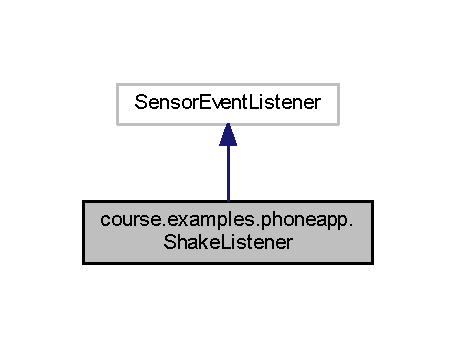
\includegraphics[width=219pt]{classcourse_1_1examples_1_1phoneapp_1_1_shake_listener__inherit__graph}
\end{center}
\end{figure}


Collaboration diagram for course.\+examples.\+phoneapp.\+Shake\+Listener\+:
\nopagebreak
\begin{figure}[H]
\begin{center}
\leavevmode
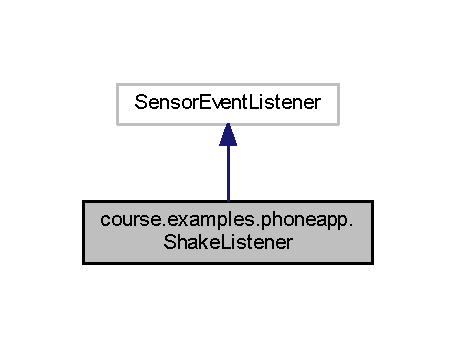
\includegraphics[width=219pt]{classcourse_1_1examples_1_1phoneapp_1_1_shake_listener__coll__graph}
\end{center}
\end{figure}
\subsection*{Classes}
\begin{DoxyCompactItemize}
\item 
interface \hyperlink{interfacecourse_1_1examples_1_1phoneapp_1_1_shake_listener_1_1_on_shake_listener}{On\+Shake\+Listener}
\end{DoxyCompactItemize}
\subsection*{Public Member Functions}
\begin{DoxyCompactItemize}
\item 
\hyperlink{classcourse_1_1examples_1_1phoneapp_1_1_shake_listener_a1ab0dfd3a0312f22d80553fc86517ef4}{Shake\+Listener} (Context context)
\item 
void \hyperlink{classcourse_1_1examples_1_1phoneapp_1_1_shake_listener_a55bc555dadb88dcb1f51b8e5e0c952cc}{set\+On\+Shake\+Listener} (\hyperlink{interfacecourse_1_1examples_1_1phoneapp_1_1_shake_listener_1_1_on_shake_listener}{On\+Shake\+Listener} listener)
\item 
void \hyperlink{classcourse_1_1examples_1_1phoneapp_1_1_shake_listener_a53d8ca8e5fda8c6b6e6fe9659d5badc9}{resume} ()
\item 
void \hyperlink{classcourse_1_1examples_1_1phoneapp_1_1_shake_listener_a5214588f55677bad1967cde68353b7ef}{pause} ()
\item 
void \hyperlink{classcourse_1_1examples_1_1phoneapp_1_1_shake_listener_a5adb466838aaee55687d30ec1d032dda}{on\+Accuracy\+Changed} (Sensor sensor, int accuracy)
\item 
void \hyperlink{classcourse_1_1examples_1_1phoneapp_1_1_shake_listener_a5faea5509575f61399e18873b33afbd0}{on\+Sensor\+Changed} (Sensor\+Event event)
\end{DoxyCompactItemize}
\subsection*{Static Public Attributes}
\begin{DoxyCompactItemize}
\item 
static final String \hyperlink{classcourse_1_1examples_1_1phoneapp_1_1_shake_listener_a6ed24cf98223b33bfa637cf67c801914}{L\+O\+G\+\_\+\+T\+A\+G\+\_\+\+N\+A\+M\+E} = \char`\"{}Phone\+App.\+Shake\+Listener\char`\"{}
\end{DoxyCompactItemize}


\subsection{Detailed Description}
Listener class to capture the shake gesture of a device and provide an event for performing any operation when triggered ~\newline
 Created by kannanb on 10/1/2015. 

\subsection{Constructor \& Destructor Documentation}
\hypertarget{classcourse_1_1examples_1_1phoneapp_1_1_shake_listener_a1ab0dfd3a0312f22d80553fc86517ef4}{}\index{course\+::examples\+::phoneapp\+::\+Shake\+Listener@{course\+::examples\+::phoneapp\+::\+Shake\+Listener}!Shake\+Listener@{Shake\+Listener}}
\index{Shake\+Listener@{Shake\+Listener}!course\+::examples\+::phoneapp\+::\+Shake\+Listener@{course\+::examples\+::phoneapp\+::\+Shake\+Listener}}
\subsubsection[{Shake\+Listener(\+Context context)}]{\setlength{\rightskip}{0pt plus 5cm}course.\+examples.\+phoneapp.\+Shake\+Listener.\+Shake\+Listener (
\begin{DoxyParamCaption}
\item[{Context}]{context}
\end{DoxyParamCaption}
)}\label{classcourse_1_1examples_1_1phoneapp_1_1_shake_listener_a1ab0dfd3a0312f22d80553fc86517ef4}
Constructor to prepare for initializing and absorbing shake event on the device 
\begin{DoxyParams}{Parameters}
{\em context} & on which the shake event is consumed \\
\hline
\end{DoxyParams}


\subsection{Member Function Documentation}
\hypertarget{classcourse_1_1examples_1_1phoneapp_1_1_shake_listener_a5adb466838aaee55687d30ec1d032dda}{}\index{course\+::examples\+::phoneapp\+::\+Shake\+Listener@{course\+::examples\+::phoneapp\+::\+Shake\+Listener}!on\+Accuracy\+Changed@{on\+Accuracy\+Changed}}
\index{on\+Accuracy\+Changed@{on\+Accuracy\+Changed}!course\+::examples\+::phoneapp\+::\+Shake\+Listener@{course\+::examples\+::phoneapp\+::\+Shake\+Listener}}
\subsubsection[{on\+Accuracy\+Changed(\+Sensor sensor, int accuracy)}]{\setlength{\rightskip}{0pt plus 5cm}void course.\+examples.\+phoneapp.\+Shake\+Listener.\+on\+Accuracy\+Changed (
\begin{DoxyParamCaption}
\item[{Sensor}]{sensor, }
\item[{int}]{accuracy}
\end{DoxyParamCaption}
)}\label{classcourse_1_1examples_1_1phoneapp_1_1_shake_listener_a5adb466838aaee55687d30ec1d032dda}
\hypertarget{classcourse_1_1examples_1_1phoneapp_1_1_shake_listener_a5faea5509575f61399e18873b33afbd0}{}\index{course\+::examples\+::phoneapp\+::\+Shake\+Listener@{course\+::examples\+::phoneapp\+::\+Shake\+Listener}!on\+Sensor\+Changed@{on\+Sensor\+Changed}}
\index{on\+Sensor\+Changed@{on\+Sensor\+Changed}!course\+::examples\+::phoneapp\+::\+Shake\+Listener@{course\+::examples\+::phoneapp\+::\+Shake\+Listener}}
\subsubsection[{on\+Sensor\+Changed(\+Sensor\+Event event)}]{\setlength{\rightskip}{0pt plus 5cm}void course.\+examples.\+phoneapp.\+Shake\+Listener.\+on\+Sensor\+Changed (
\begin{DoxyParamCaption}
\item[{Sensor\+Event}]{event}
\end{DoxyParamCaption}
)}\label{classcourse_1_1examples_1_1phoneapp_1_1_shake_listener_a5faea5509575f61399e18873b33afbd0}
Method to perform calculation on how to detect a shake of a device by the user 
\begin{DoxyParams}{Parameters}
{\em event} & \\
\hline
\end{DoxyParams}
\hypertarget{classcourse_1_1examples_1_1phoneapp_1_1_shake_listener_a5214588f55677bad1967cde68353b7ef}{}\index{course\+::examples\+::phoneapp\+::\+Shake\+Listener@{course\+::examples\+::phoneapp\+::\+Shake\+Listener}!pause@{pause}}
\index{pause@{pause}!course\+::examples\+::phoneapp\+::\+Shake\+Listener@{course\+::examples\+::phoneapp\+::\+Shake\+Listener}}
\subsubsection[{pause()}]{\setlength{\rightskip}{0pt plus 5cm}void course.\+examples.\+phoneapp.\+Shake\+Listener.\+pause (
\begin{DoxyParamCaption}
{}
\end{DoxyParamCaption}
)}\label{classcourse_1_1examples_1_1phoneapp_1_1_shake_listener_a5214588f55677bad1967cde68353b7ef}
Method to unregister the sensor when the activity has been paused. This will save battery power \hypertarget{classcourse_1_1examples_1_1phoneapp_1_1_shake_listener_a53d8ca8e5fda8c6b6e6fe9659d5badc9}{}\index{course\+::examples\+::phoneapp\+::\+Shake\+Listener@{course\+::examples\+::phoneapp\+::\+Shake\+Listener}!resume@{resume}}
\index{resume@{resume}!course\+::examples\+::phoneapp\+::\+Shake\+Listener@{course\+::examples\+::phoneapp\+::\+Shake\+Listener}}
\subsubsection[{resume()}]{\setlength{\rightskip}{0pt plus 5cm}void course.\+examples.\+phoneapp.\+Shake\+Listener.\+resume (
\begin{DoxyParamCaption}
{}
\end{DoxyParamCaption}
)}\label{classcourse_1_1examples_1_1phoneapp_1_1_shake_listener_a53d8ca8e5fda8c6b6e6fe9659d5badc9}
Method to register the Accerlerometer Sensor to help sense the shake of the device \hypertarget{classcourse_1_1examples_1_1phoneapp_1_1_shake_listener_a55bc555dadb88dcb1f51b8e5e0c952cc}{}\index{course\+::examples\+::phoneapp\+::\+Shake\+Listener@{course\+::examples\+::phoneapp\+::\+Shake\+Listener}!set\+On\+Shake\+Listener@{set\+On\+Shake\+Listener}}
\index{set\+On\+Shake\+Listener@{set\+On\+Shake\+Listener}!course\+::examples\+::phoneapp\+::\+Shake\+Listener@{course\+::examples\+::phoneapp\+::\+Shake\+Listener}}
\subsubsection[{set\+On\+Shake\+Listener(\+On\+Shake\+Listener listener)}]{\setlength{\rightskip}{0pt plus 5cm}void course.\+examples.\+phoneapp.\+Shake\+Listener.\+set\+On\+Shake\+Listener (
\begin{DoxyParamCaption}
\item[{{\bf On\+Shake\+Listener}}]{listener}
\end{DoxyParamCaption}
)}\label{classcourse_1_1examples_1_1phoneapp_1_1_shake_listener_a55bc555dadb88dcb1f51b8e5e0c952cc}
Method to set the user defined \hyperlink{interfacecourse_1_1examples_1_1phoneapp_1_1_shake_listener_1_1_on_shake_listener}{On\+Shake\+Listener} 
\begin{DoxyParams}{Parameters}
{\em listener} & interested in the shake event of the device \\
\hline
\end{DoxyParams}


\subsection{Member Data Documentation}
\hypertarget{classcourse_1_1examples_1_1phoneapp_1_1_shake_listener_a6ed24cf98223b33bfa637cf67c801914}{}\index{course\+::examples\+::phoneapp\+::\+Shake\+Listener@{course\+::examples\+::phoneapp\+::\+Shake\+Listener}!L\+O\+G\+\_\+\+T\+A\+G\+\_\+\+N\+A\+M\+E@{L\+O\+G\+\_\+\+T\+A\+G\+\_\+\+N\+A\+M\+E}}
\index{L\+O\+G\+\_\+\+T\+A\+G\+\_\+\+N\+A\+M\+E@{L\+O\+G\+\_\+\+T\+A\+G\+\_\+\+N\+A\+M\+E}!course\+::examples\+::phoneapp\+::\+Shake\+Listener@{course\+::examples\+::phoneapp\+::\+Shake\+Listener}}
\subsubsection[{L\+O\+G\+\_\+\+T\+A\+G\+\_\+\+N\+A\+M\+E}]{\setlength{\rightskip}{0pt plus 5cm}final String course.\+examples.\+phoneapp.\+Shake\+Listener.\+L\+O\+G\+\_\+\+T\+A\+G\+\_\+\+N\+A\+M\+E = \char`\"{}Phone\+App.\+Shake\+Listener\char`\"{}\hspace{0.3cm}{\ttfamily [static]}}\label{classcourse_1_1examples_1_1phoneapp_1_1_shake_listener_a6ed24cf98223b33bfa637cf67c801914}


The documentation for this class was generated from the following file\+:\begin{DoxyCompactItemize}
\item 
app/src/main/java/course/examples/phoneapp/\hyperlink{_shake_listener_8java}{Shake\+Listener.\+java}\end{DoxyCompactItemize}

\hypertarget{classcourse_1_1examples_1_1phoneapp_1_1_utility}{}\section{course.\+examples.\+phoneapp.\+Utility Class Reference}
\label{classcourse_1_1examples_1_1phoneapp_1_1_utility}\index{course.\+examples.\+phoneapp.\+Utility@{course.\+examples.\+phoneapp.\+Utility}}
\subsection*{Classes}
\begin{DoxyCompactItemize}
\item 
class {\bfseries Download\+File}
\item 
class {\bfseries Update\+List}
\item 
class {\bfseries Upload\+File}
\end{DoxyCompactItemize}
\subsection*{Static Public Member Functions}
\begin{DoxyCompactItemize}
\item 
static void \hyperlink{classcourse_1_1examples_1_1phoneapp_1_1_utility_a79e295a2526fd5fa44894beeca99f340}{show\+Toast} (Context context, String message)
\item 
static void \hyperlink{classcourse_1_1examples_1_1phoneapp_1_1_utility_a5f33366b0ef1f6e6cc3e25c35dc1e0b6}{send\+S\+M\+S} (String phone\+Number, String msg\+Body, String mime\+Type, Context context)
\item 
static void \hyperlink{classcourse_1_1examples_1_1phoneapp_1_1_utility_a8b997770364b4ae7620db3e18716ec2d}{send\+S\+M\+S\+Whats\+App} (String phone\+Number, String msg\+Body, String mime\+Type, String package\+Name, Context context)
\item 
static void \hyperlink{classcourse_1_1examples_1_1phoneapp_1_1_utility_a1435fdd4dd435034a5d866a6d586e68a}{send\+Email} (String subject, String msg\+Body, String from, String to, String cc, Context context)
\item 
static void \hyperlink{classcourse_1_1examples_1_1phoneapp_1_1_utility_a6532b2cd02df1fa71b50362636401628}{phone\+Call} (String phone\+Number, Context context)
\item 
static void \hyperlink{classcourse_1_1examples_1_1phoneapp_1_1_utility_a52a9f17fcb5689b3da8038811ee6abf4}{alert} (String msg\+Body, String title, Context context)
\item 
static int \hyperlink{classcourse_1_1examples_1_1phoneapp_1_1_utility_a01fad705fa764f0d337f90069427ffb5}{confirm\+Dialog} (String msg\+Body, String title, Context context)
\item 
static List$<$ String $>$ \hyperlink{classcourse_1_1examples_1_1phoneapp_1_1_utility_a578fd485bd50d243570a8eed4af04bc9}{read\+Phone\+List\+From\+File} (File file)
\item 
static List$<$ String $>$ \hyperlink{classcourse_1_1examples_1_1phoneapp_1_1_utility_ab87f4ad40f39634a8705bb47ae674727}{get\+Phone\+Contacts\+Ex} (Context context)
\item 
static void \hyperlink{classcourse_1_1examples_1_1phoneapp_1_1_utility_a1e30a36857885efeacdf33996403a26f}{update\+Phone\+D\+B} (List$<$ String $>$ list, Context context)
\item 
static List$<$ String $>$ \hyperlink{classcourse_1_1examples_1_1phoneapp_1_1_utility_a5ef96751af1965557ef365d7426044fa}{get\+Phone\+Contacts} (Context c)
\item 
static List$<$ String $>$ \hyperlink{classcourse_1_1examples_1_1phoneapp_1_1_utility_aa34007fd1fb09ca6de7861b30690c942}{get\+Detailed\+Phone\+Contacts} (Context c)
\end{DoxyCompactItemize}
\subsection*{Static Public Attributes}
\begin{DoxyCompactItemize}
\item 
static final String \hyperlink{classcourse_1_1examples_1_1phoneapp_1_1_utility_a35835b9e24f4150c50657a03448919da}{T\+E\+X\+T\+\_\+\+M\+I\+M\+E\+\_\+\+T\+Y\+P\+E} = \char`\"{}text/plain\char`\"{}
\item 
static final String \hyperlink{classcourse_1_1examples_1_1phoneapp_1_1_utility_a6b677db05046c2fcb1b6770f39bf35f2}{S\+M\+S\+\_\+\+M\+I\+M\+E\+\_\+\+T\+Y\+P\+E} = \char`\"{}vnd.\+android-\/dir/mms-\/sms\char`\"{}
\item 
static final String \hyperlink{classcourse_1_1examples_1_1phoneapp_1_1_utility_ade5eb8c8a3772fbacb49d38f450ca9b5}{W\+H\+A\+T\+S\+A\+P\+P\+\_\+\+P\+A\+C\+K\+A\+G\+E\+\_\+\+N\+A\+M\+E} = \char`\"{}com.\+whatsapp\char`\"{}
\item 
static final String \hyperlink{classcourse_1_1examples_1_1phoneapp_1_1_utility_a91b350654a317da65ecc2bebda4129f7}{L\+O\+G\+\_\+\+T\+A\+G\+\_\+\+N\+A\+M\+E} = \char`\"{}Kannan\char`\"{}
\item 
static final String \hyperlink{classcourse_1_1examples_1_1phoneapp_1_1_utility_a7712af7f884a75deb1272dddc4bf5dc9}{D\+E\+L\+I\+M\+I\+T\+E\+R} = \char`\"{};\char`\"{}
\end{DoxyCompactItemize}


\subsection{Detailed Description}
Created by kannanb on 9/29/2015. 

\subsection{Member Function Documentation}
\hypertarget{classcourse_1_1examples_1_1phoneapp_1_1_utility_a52a9f17fcb5689b3da8038811ee6abf4}{}\index{course\+::examples\+::phoneapp\+::\+Utility@{course\+::examples\+::phoneapp\+::\+Utility}!alert@{alert}}
\index{alert@{alert}!course\+::examples\+::phoneapp\+::\+Utility@{course\+::examples\+::phoneapp\+::\+Utility}}
\subsubsection[{alert(\+String msg\+Body, String title, Context context)}]{\setlength{\rightskip}{0pt plus 5cm}static void course.\+examples.\+phoneapp.\+Utility.\+alert (
\begin{DoxyParamCaption}
\item[{String}]{msg\+Body, }
\item[{String}]{title, }
\item[{Context}]{context}
\end{DoxyParamCaption}
)\hspace{0.3cm}{\ttfamily [static]}}\label{classcourse_1_1examples_1_1phoneapp_1_1_utility_a52a9f17fcb5689b3da8038811ee6abf4}
\hypertarget{classcourse_1_1examples_1_1phoneapp_1_1_utility_a01fad705fa764f0d337f90069427ffb5}{}\index{course\+::examples\+::phoneapp\+::\+Utility@{course\+::examples\+::phoneapp\+::\+Utility}!confirm\+Dialog@{confirm\+Dialog}}
\index{confirm\+Dialog@{confirm\+Dialog}!course\+::examples\+::phoneapp\+::\+Utility@{course\+::examples\+::phoneapp\+::\+Utility}}
\subsubsection[{confirm\+Dialog(\+String msg\+Body, String title, Context context)}]{\setlength{\rightskip}{0pt plus 5cm}static int course.\+examples.\+phoneapp.\+Utility.\+confirm\+Dialog (
\begin{DoxyParamCaption}
\item[{String}]{msg\+Body, }
\item[{String}]{title, }
\item[{Context}]{context}
\end{DoxyParamCaption}
)\hspace{0.3cm}{\ttfamily [static]}}\label{classcourse_1_1examples_1_1phoneapp_1_1_utility_a01fad705fa764f0d337f90069427ffb5}
\hypertarget{classcourse_1_1examples_1_1phoneapp_1_1_utility_aa34007fd1fb09ca6de7861b30690c942}{}\index{course\+::examples\+::phoneapp\+::\+Utility@{course\+::examples\+::phoneapp\+::\+Utility}!get\+Detailed\+Phone\+Contacts@{get\+Detailed\+Phone\+Contacts}}
\index{get\+Detailed\+Phone\+Contacts@{get\+Detailed\+Phone\+Contacts}!course\+::examples\+::phoneapp\+::\+Utility@{course\+::examples\+::phoneapp\+::\+Utility}}
\subsubsection[{get\+Detailed\+Phone\+Contacts(\+Context c)}]{\setlength{\rightskip}{0pt plus 5cm}static List$<$String$>$ course.\+examples.\+phoneapp.\+Utility.\+get\+Detailed\+Phone\+Contacts (
\begin{DoxyParamCaption}
\item[{Context}]{c}
\end{DoxyParamCaption}
)\hspace{0.3cm}{\ttfamily [static]}}\label{classcourse_1_1examples_1_1phoneapp_1_1_utility_aa34007fd1fb09ca6de7861b30690c942}
\hypertarget{classcourse_1_1examples_1_1phoneapp_1_1_utility_a5ef96751af1965557ef365d7426044fa}{}\index{course\+::examples\+::phoneapp\+::\+Utility@{course\+::examples\+::phoneapp\+::\+Utility}!get\+Phone\+Contacts@{get\+Phone\+Contacts}}
\index{get\+Phone\+Contacts@{get\+Phone\+Contacts}!course\+::examples\+::phoneapp\+::\+Utility@{course\+::examples\+::phoneapp\+::\+Utility}}
\subsubsection[{get\+Phone\+Contacts(\+Context c)}]{\setlength{\rightskip}{0pt plus 5cm}static List$<$String$>$ course.\+examples.\+phoneapp.\+Utility.\+get\+Phone\+Contacts (
\begin{DoxyParamCaption}
\item[{Context}]{c}
\end{DoxyParamCaption}
)\hspace{0.3cm}{\ttfamily [static]}}\label{classcourse_1_1examples_1_1phoneapp_1_1_utility_a5ef96751af1965557ef365d7426044fa}
\hypertarget{classcourse_1_1examples_1_1phoneapp_1_1_utility_ab87f4ad40f39634a8705bb47ae674727}{}\index{course\+::examples\+::phoneapp\+::\+Utility@{course\+::examples\+::phoneapp\+::\+Utility}!get\+Phone\+Contacts\+Ex@{get\+Phone\+Contacts\+Ex}}
\index{get\+Phone\+Contacts\+Ex@{get\+Phone\+Contacts\+Ex}!course\+::examples\+::phoneapp\+::\+Utility@{course\+::examples\+::phoneapp\+::\+Utility}}
\subsubsection[{get\+Phone\+Contacts\+Ex(\+Context context)}]{\setlength{\rightskip}{0pt plus 5cm}static List$<$String$>$ course.\+examples.\+phoneapp.\+Utility.\+get\+Phone\+Contacts\+Ex (
\begin{DoxyParamCaption}
\item[{Context}]{context}
\end{DoxyParamCaption}
)\hspace{0.3cm}{\ttfamily [static]}}\label{classcourse_1_1examples_1_1phoneapp_1_1_utility_ab87f4ad40f39634a8705bb47ae674727}
\hypertarget{classcourse_1_1examples_1_1phoneapp_1_1_utility_a6532b2cd02df1fa71b50362636401628}{}\index{course\+::examples\+::phoneapp\+::\+Utility@{course\+::examples\+::phoneapp\+::\+Utility}!phone\+Call@{phone\+Call}}
\index{phone\+Call@{phone\+Call}!course\+::examples\+::phoneapp\+::\+Utility@{course\+::examples\+::phoneapp\+::\+Utility}}
\subsubsection[{phone\+Call(\+String phone\+Number, Context context)}]{\setlength{\rightskip}{0pt plus 5cm}static void course.\+examples.\+phoneapp.\+Utility.\+phone\+Call (
\begin{DoxyParamCaption}
\item[{String}]{phone\+Number, }
\item[{Context}]{context}
\end{DoxyParamCaption}
)\hspace{0.3cm}{\ttfamily [static]}}\label{classcourse_1_1examples_1_1phoneapp_1_1_utility_a6532b2cd02df1fa71b50362636401628}
\hypertarget{classcourse_1_1examples_1_1phoneapp_1_1_utility_a578fd485bd50d243570a8eed4af04bc9}{}\index{course\+::examples\+::phoneapp\+::\+Utility@{course\+::examples\+::phoneapp\+::\+Utility}!read\+Phone\+List\+From\+File@{read\+Phone\+List\+From\+File}}
\index{read\+Phone\+List\+From\+File@{read\+Phone\+List\+From\+File}!course\+::examples\+::phoneapp\+::\+Utility@{course\+::examples\+::phoneapp\+::\+Utility}}
\subsubsection[{read\+Phone\+List\+From\+File(\+File file)}]{\setlength{\rightskip}{0pt plus 5cm}static List$<$String$>$ course.\+examples.\+phoneapp.\+Utility.\+read\+Phone\+List\+From\+File (
\begin{DoxyParamCaption}
\item[{File}]{file}
\end{DoxyParamCaption}
)\hspace{0.3cm}{\ttfamily [static]}}\label{classcourse_1_1examples_1_1phoneapp_1_1_utility_a578fd485bd50d243570a8eed4af04bc9}
\hypertarget{classcourse_1_1examples_1_1phoneapp_1_1_utility_a1435fdd4dd435034a5d866a6d586e68a}{}\index{course\+::examples\+::phoneapp\+::\+Utility@{course\+::examples\+::phoneapp\+::\+Utility}!send\+Email@{send\+Email}}
\index{send\+Email@{send\+Email}!course\+::examples\+::phoneapp\+::\+Utility@{course\+::examples\+::phoneapp\+::\+Utility}}
\subsubsection[{send\+Email(\+String subject, String msg\+Body, String from, String to, String cc, Context context)}]{\setlength{\rightskip}{0pt plus 5cm}static void course.\+examples.\+phoneapp.\+Utility.\+send\+Email (
\begin{DoxyParamCaption}
\item[{String}]{subject, }
\item[{String}]{msg\+Body, }
\item[{String}]{from, }
\item[{String}]{to, }
\item[{String}]{cc, }
\item[{Context}]{context}
\end{DoxyParamCaption}
)\hspace{0.3cm}{\ttfamily [static]}}\label{classcourse_1_1examples_1_1phoneapp_1_1_utility_a1435fdd4dd435034a5d866a6d586e68a}
\hypertarget{classcourse_1_1examples_1_1phoneapp_1_1_utility_a5f33366b0ef1f6e6cc3e25c35dc1e0b6}{}\index{course\+::examples\+::phoneapp\+::\+Utility@{course\+::examples\+::phoneapp\+::\+Utility}!send\+S\+M\+S@{send\+S\+M\+S}}
\index{send\+S\+M\+S@{send\+S\+M\+S}!course\+::examples\+::phoneapp\+::\+Utility@{course\+::examples\+::phoneapp\+::\+Utility}}
\subsubsection[{send\+S\+M\+S(\+String phone\+Number, String msg\+Body, String mime\+Type, Context context)}]{\setlength{\rightskip}{0pt plus 5cm}static void course.\+examples.\+phoneapp.\+Utility.\+send\+S\+M\+S (
\begin{DoxyParamCaption}
\item[{String}]{phone\+Number, }
\item[{String}]{msg\+Body, }
\item[{String}]{mime\+Type, }
\item[{Context}]{context}
\end{DoxyParamCaption}
)\hspace{0.3cm}{\ttfamily [static]}}\label{classcourse_1_1examples_1_1phoneapp_1_1_utility_a5f33366b0ef1f6e6cc3e25c35dc1e0b6}
\hypertarget{classcourse_1_1examples_1_1phoneapp_1_1_utility_a8b997770364b4ae7620db3e18716ec2d}{}\index{course\+::examples\+::phoneapp\+::\+Utility@{course\+::examples\+::phoneapp\+::\+Utility}!send\+S\+M\+S\+Whats\+App@{send\+S\+M\+S\+Whats\+App}}
\index{send\+S\+M\+S\+Whats\+App@{send\+S\+M\+S\+Whats\+App}!course\+::examples\+::phoneapp\+::\+Utility@{course\+::examples\+::phoneapp\+::\+Utility}}
\subsubsection[{send\+S\+M\+S\+Whats\+App(\+String phone\+Number, String msg\+Body, String mime\+Type, String package\+Name, Context context)}]{\setlength{\rightskip}{0pt plus 5cm}static void course.\+examples.\+phoneapp.\+Utility.\+send\+S\+M\+S\+Whats\+App (
\begin{DoxyParamCaption}
\item[{String}]{phone\+Number, }
\item[{String}]{msg\+Body, }
\item[{String}]{mime\+Type, }
\item[{String}]{package\+Name, }
\item[{Context}]{context}
\end{DoxyParamCaption}
)\hspace{0.3cm}{\ttfamily [static]}}\label{classcourse_1_1examples_1_1phoneapp_1_1_utility_a8b997770364b4ae7620db3e18716ec2d}
\hypertarget{classcourse_1_1examples_1_1phoneapp_1_1_utility_a79e295a2526fd5fa44894beeca99f340}{}\index{course\+::examples\+::phoneapp\+::\+Utility@{course\+::examples\+::phoneapp\+::\+Utility}!show\+Toast@{show\+Toast}}
\index{show\+Toast@{show\+Toast}!course\+::examples\+::phoneapp\+::\+Utility@{course\+::examples\+::phoneapp\+::\+Utility}}
\subsubsection[{show\+Toast(\+Context context, String message)}]{\setlength{\rightskip}{0pt plus 5cm}static void course.\+examples.\+phoneapp.\+Utility.\+show\+Toast (
\begin{DoxyParamCaption}
\item[{Context}]{context, }
\item[{String}]{message}
\end{DoxyParamCaption}
)\hspace{0.3cm}{\ttfamily [static]}}\label{classcourse_1_1examples_1_1phoneapp_1_1_utility_a79e295a2526fd5fa44894beeca99f340}
\hypertarget{classcourse_1_1examples_1_1phoneapp_1_1_utility_a1e30a36857885efeacdf33996403a26f}{}\index{course\+::examples\+::phoneapp\+::\+Utility@{course\+::examples\+::phoneapp\+::\+Utility}!update\+Phone\+D\+B@{update\+Phone\+D\+B}}
\index{update\+Phone\+D\+B@{update\+Phone\+D\+B}!course\+::examples\+::phoneapp\+::\+Utility@{course\+::examples\+::phoneapp\+::\+Utility}}
\subsubsection[{update\+Phone\+D\+B(\+List$<$ String $>$ list, Context context)}]{\setlength{\rightskip}{0pt plus 5cm}static void course.\+examples.\+phoneapp.\+Utility.\+update\+Phone\+D\+B (
\begin{DoxyParamCaption}
\item[{List$<$ String $>$}]{list, }
\item[{Context}]{context}
\end{DoxyParamCaption}
)\hspace{0.3cm}{\ttfamily [static]}}\label{classcourse_1_1examples_1_1phoneapp_1_1_utility_a1e30a36857885efeacdf33996403a26f}


\subsection{Member Data Documentation}
\hypertarget{classcourse_1_1examples_1_1phoneapp_1_1_utility_a7712af7f884a75deb1272dddc4bf5dc9}{}\index{course\+::examples\+::phoneapp\+::\+Utility@{course\+::examples\+::phoneapp\+::\+Utility}!D\+E\+L\+I\+M\+I\+T\+E\+R@{D\+E\+L\+I\+M\+I\+T\+E\+R}}
\index{D\+E\+L\+I\+M\+I\+T\+E\+R@{D\+E\+L\+I\+M\+I\+T\+E\+R}!course\+::examples\+::phoneapp\+::\+Utility@{course\+::examples\+::phoneapp\+::\+Utility}}
\subsubsection[{D\+E\+L\+I\+M\+I\+T\+E\+R}]{\setlength{\rightskip}{0pt plus 5cm}final String course.\+examples.\+phoneapp.\+Utility.\+D\+E\+L\+I\+M\+I\+T\+E\+R = \char`\"{};\char`\"{}\hspace{0.3cm}{\ttfamily [static]}}\label{classcourse_1_1examples_1_1phoneapp_1_1_utility_a7712af7f884a75deb1272dddc4bf5dc9}
\hypertarget{classcourse_1_1examples_1_1phoneapp_1_1_utility_a91b350654a317da65ecc2bebda4129f7}{}\index{course\+::examples\+::phoneapp\+::\+Utility@{course\+::examples\+::phoneapp\+::\+Utility}!L\+O\+G\+\_\+\+T\+A\+G\+\_\+\+N\+A\+M\+E@{L\+O\+G\+\_\+\+T\+A\+G\+\_\+\+N\+A\+M\+E}}
\index{L\+O\+G\+\_\+\+T\+A\+G\+\_\+\+N\+A\+M\+E@{L\+O\+G\+\_\+\+T\+A\+G\+\_\+\+N\+A\+M\+E}!course\+::examples\+::phoneapp\+::\+Utility@{course\+::examples\+::phoneapp\+::\+Utility}}
\subsubsection[{L\+O\+G\+\_\+\+T\+A\+G\+\_\+\+N\+A\+M\+E}]{\setlength{\rightskip}{0pt plus 5cm}final String course.\+examples.\+phoneapp.\+Utility.\+L\+O\+G\+\_\+\+T\+A\+G\+\_\+\+N\+A\+M\+E = \char`\"{}Kannan\char`\"{}\hspace{0.3cm}{\ttfamily [static]}}\label{classcourse_1_1examples_1_1phoneapp_1_1_utility_a91b350654a317da65ecc2bebda4129f7}
\hypertarget{classcourse_1_1examples_1_1phoneapp_1_1_utility_a6b677db05046c2fcb1b6770f39bf35f2}{}\index{course\+::examples\+::phoneapp\+::\+Utility@{course\+::examples\+::phoneapp\+::\+Utility}!S\+M\+S\+\_\+\+M\+I\+M\+E\+\_\+\+T\+Y\+P\+E@{S\+M\+S\+\_\+\+M\+I\+M\+E\+\_\+\+T\+Y\+P\+E}}
\index{S\+M\+S\+\_\+\+M\+I\+M\+E\+\_\+\+T\+Y\+P\+E@{S\+M\+S\+\_\+\+M\+I\+M\+E\+\_\+\+T\+Y\+P\+E}!course\+::examples\+::phoneapp\+::\+Utility@{course\+::examples\+::phoneapp\+::\+Utility}}
\subsubsection[{S\+M\+S\+\_\+\+M\+I\+M\+E\+\_\+\+T\+Y\+P\+E}]{\setlength{\rightskip}{0pt plus 5cm}final String course.\+examples.\+phoneapp.\+Utility.\+S\+M\+S\+\_\+\+M\+I\+M\+E\+\_\+\+T\+Y\+P\+E = \char`\"{}vnd.\+android-\/dir/mms-\/sms\char`\"{}\hspace{0.3cm}{\ttfamily [static]}}\label{classcourse_1_1examples_1_1phoneapp_1_1_utility_a6b677db05046c2fcb1b6770f39bf35f2}
\hypertarget{classcourse_1_1examples_1_1phoneapp_1_1_utility_a35835b9e24f4150c50657a03448919da}{}\index{course\+::examples\+::phoneapp\+::\+Utility@{course\+::examples\+::phoneapp\+::\+Utility}!T\+E\+X\+T\+\_\+\+M\+I\+M\+E\+\_\+\+T\+Y\+P\+E@{T\+E\+X\+T\+\_\+\+M\+I\+M\+E\+\_\+\+T\+Y\+P\+E}}
\index{T\+E\+X\+T\+\_\+\+M\+I\+M\+E\+\_\+\+T\+Y\+P\+E@{T\+E\+X\+T\+\_\+\+M\+I\+M\+E\+\_\+\+T\+Y\+P\+E}!course\+::examples\+::phoneapp\+::\+Utility@{course\+::examples\+::phoneapp\+::\+Utility}}
\subsubsection[{T\+E\+X\+T\+\_\+\+M\+I\+M\+E\+\_\+\+T\+Y\+P\+E}]{\setlength{\rightskip}{0pt plus 5cm}final String course.\+examples.\+phoneapp.\+Utility.\+T\+E\+X\+T\+\_\+\+M\+I\+M\+E\+\_\+\+T\+Y\+P\+E = \char`\"{}text/plain\char`\"{}\hspace{0.3cm}{\ttfamily [static]}}\label{classcourse_1_1examples_1_1phoneapp_1_1_utility_a35835b9e24f4150c50657a03448919da}
\hypertarget{classcourse_1_1examples_1_1phoneapp_1_1_utility_ade5eb8c8a3772fbacb49d38f450ca9b5}{}\index{course\+::examples\+::phoneapp\+::\+Utility@{course\+::examples\+::phoneapp\+::\+Utility}!W\+H\+A\+T\+S\+A\+P\+P\+\_\+\+P\+A\+C\+K\+A\+G\+E\+\_\+\+N\+A\+M\+E@{W\+H\+A\+T\+S\+A\+P\+P\+\_\+\+P\+A\+C\+K\+A\+G\+E\+\_\+\+N\+A\+M\+E}}
\index{W\+H\+A\+T\+S\+A\+P\+P\+\_\+\+P\+A\+C\+K\+A\+G\+E\+\_\+\+N\+A\+M\+E@{W\+H\+A\+T\+S\+A\+P\+P\+\_\+\+P\+A\+C\+K\+A\+G\+E\+\_\+\+N\+A\+M\+E}!course\+::examples\+::phoneapp\+::\+Utility@{course\+::examples\+::phoneapp\+::\+Utility}}
\subsubsection[{W\+H\+A\+T\+S\+A\+P\+P\+\_\+\+P\+A\+C\+K\+A\+G\+E\+\_\+\+N\+A\+M\+E}]{\setlength{\rightskip}{0pt plus 5cm}final String course.\+examples.\+phoneapp.\+Utility.\+W\+H\+A\+T\+S\+A\+P\+P\+\_\+\+P\+A\+C\+K\+A\+G\+E\+\_\+\+N\+A\+M\+E = \char`\"{}com.\+whatsapp\char`\"{}\hspace{0.3cm}{\ttfamily [static]}}\label{classcourse_1_1examples_1_1phoneapp_1_1_utility_ade5eb8c8a3772fbacb49d38f450ca9b5}


The documentation for this class was generated from the following file\+:\begin{DoxyCompactItemize}
\item 
app/src/main/java/course/examples/phoneapp/\hyperlink{_utility_8java}{Utility.\+java}\end{DoxyCompactItemize}

\chapter{File Documentation}
\hypertarget{_contact___details_8java}{}\section{app/src/main/java/course/examples/phoneapp/\+Contact\+\_\+\+Details.java File Reference}
\label{_contact___details_8java}\index{app/src/main/java/course/examples/phoneapp/\+Contact\+\_\+\+Details.\+java@{app/src/main/java/course/examples/phoneapp/\+Contact\+\_\+\+Details.\+java}}
\subsection*{Classes}
\begin{DoxyCompactItemize}
\item 
class \hyperlink{classcourse_1_1examples_1_1phoneapp_1_1_contact___details}{course.\+examples.\+phoneapp.\+Contact\+\_\+\+Details}
\end{DoxyCompactItemize}
\subsection*{Packages}
\begin{DoxyCompactItemize}
\item 
package \hyperlink{namespacecourse_1_1examples_1_1phoneapp}{course.\+examples.\+phoneapp}
\end{DoxyCompactItemize}

\hypertarget{_main_activity_8java}{}\section{app/src/main/java/course/examples/phoneapp/\+Main\+Activity.java File Reference}
\label{_main_activity_8java}\index{app/src/main/java/course/examples/phoneapp/\+Main\+Activity.\+java@{app/src/main/java/course/examples/phoneapp/\+Main\+Activity.\+java}}
\subsection*{Classes}
\begin{DoxyCompactItemize}
\item 
class \hyperlink{classcourse_1_1examples_1_1phoneapp_1_1_main_activity}{course.\+examples.\+phoneapp.\+Main\+Activity}
\end{DoxyCompactItemize}
\subsection*{Packages}
\begin{DoxyCompactItemize}
\item 
package \hyperlink{namespacecourse_1_1examples_1_1phoneapp}{course.\+examples.\+phoneapp}
\end{DoxyCompactItemize}

\hypertarget{_ops_activity_8java}{}\section{app/src/main/java/course/examples/phoneapp/\+Ops\+Activity.java File Reference}
\label{_ops_activity_8java}\index{app/src/main/java/course/examples/phoneapp/\+Ops\+Activity.\+java@{app/src/main/java/course/examples/phoneapp/\+Ops\+Activity.\+java}}
\subsection*{Classes}
\begin{DoxyCompactItemize}
\item 
class \hyperlink{classcourse_1_1examples_1_1phoneapp_1_1_ops_activity}{course.\+examples.\+phoneapp.\+Ops\+Activity}
\end{DoxyCompactItemize}
\subsection*{Packages}
\begin{DoxyCompactItemize}
\item 
package \hyperlink{namespacecourse_1_1examples_1_1phoneapp}{course.\+examples.\+phoneapp}
\end{DoxyCompactItemize}

\hypertarget{_shake_listener_8java}{}\section{app/src/main/java/course/examples/phoneapp/\+Shake\+Listener.java File Reference}
\label{_shake_listener_8java}\index{app/src/main/java/course/examples/phoneapp/\+Shake\+Listener.\+java@{app/src/main/java/course/examples/phoneapp/\+Shake\+Listener.\+java}}
\subsection*{Classes}
\begin{DoxyCompactItemize}
\item 
class \hyperlink{classcourse_1_1examples_1_1phoneapp_1_1_shake_listener}{course.\+examples.\+phoneapp.\+Shake\+Listener}
\item 
interface \hyperlink{interfacecourse_1_1examples_1_1phoneapp_1_1_shake_listener_1_1_on_shake_listener}{course.\+examples.\+phoneapp.\+Shake\+Listener.\+On\+Shake\+Listener}
\end{DoxyCompactItemize}
\subsection*{Packages}
\begin{DoxyCompactItemize}
\item 
package \hyperlink{namespacecourse_1_1examples_1_1phoneapp}{course.\+examples.\+phoneapp}
\end{DoxyCompactItemize}

\hypertarget{_utility_8java}{}\section{app/src/main/java/course/examples/phoneapp/\+Utility.java File Reference}
\label{_utility_8java}\index{app/src/main/java/course/examples/phoneapp/\+Utility.\+java@{app/src/main/java/course/examples/phoneapp/\+Utility.\+java}}
\subsection*{Classes}
\begin{DoxyCompactItemize}
\item 
class \hyperlink{classcourse_1_1examples_1_1phoneapp_1_1_utility}{course.\+examples.\+phoneapp.\+Utility}
\item 
class {\bfseries course.\+examples.\+phoneapp.\+Utility.\+Upload\+File}
\item 
class {\bfseries course.\+examples.\+phoneapp.\+Utility.\+Download\+File}
\item 
class {\bfseries course.\+examples.\+phoneapp.\+Utility.\+Update\+List}
\end{DoxyCompactItemize}
\subsection*{Packages}
\begin{DoxyCompactItemize}
\item 
package \hyperlink{namespacecourse_1_1examples_1_1phoneapp}{course.\+examples.\+phoneapp}
\end{DoxyCompactItemize}

%--- End generated contents ---

% Index
\backmatter
\newpage
\phantomsection
\clearemptydoublepage
\addcontentsline{toc}{chapter}{Index}
\printindex

\end{document}
